%=======================================================================
%  Satellite embeddings, text and night lights for municipal GDP -- final talk: the work since the mid-term
%  Plan: PLAN_final_talk.md. Research only (no application). Same design as the mid-term deck, whose assets it
%  reuses. A chip in the top-right corner marks each slide as a recap (before the mid-term) or new work.
%  Footer route line: Objective, Recap, Robustness, Errors, Embeddings, Transfer, Wrap-up.
%  Build (XeLaTeX, Lato; uses the system font or MiKTeX's Lato files):
%     cd presentation/final && latexmk -xelatex final_talk.tex
%=======================================================================
\documentclass[aspectratio=169,10pt]{beamer}
\usefonttheme{professionalfonts}
\usepackage{fontspec}
\IfFontExistsTF{Lato}{%
  \setsansfont{Lato}\newfontfamily\blackfont{Lato Black}\newfontfamily\lightfont{Lato Light}}{%
  \setsansfont{Lato-Regular.ttf}[BoldFont=Lato-Bold.ttf,ItalicFont=Lato-Italic.ttf,BoldItalicFont=Lato-BoldItalic.ttf]
  \newfontfamily\blackfont{Lato-Black.ttf}\newfontfamily\lightfont{Lato-Light.ttf}}
\usepackage{amsmath,amssymb}
\usepackage{booktabs,array,graphicx,xcolor}
\usepackage[normalem]{ulem}
\usepackage{tikz}
\usetikzlibrary{arrows.meta,positioning,calc,fit,backgrounds}
\graphicspath{{assets/}{../midterm/assets/}{../../reports/figures/}}

%------------------------- palette (same hex as make_figures.py) --------
\definecolor{night}{HTML}{0B1328}
\definecolor{night2}{HTML}{16223F}
\definecolor{glow}{HTML}{F2B134}
\definecolor{paper}{HTML}{F7F5F0}
\definecolor{ink}{HTML}{1E2433}
\definecolor{muted}{HTML}{687082}
\definecolor{rule}{HTML}{D9D5CC}
\definecolor{cimg}{HTML}{138A8A}
\definecolor{ctxt}{HTML}{7057C9}
\definecolor{cntl}{HTML}{E19A1F}
\definecolor{cgdp}{HTML}{C4493B}
\definecolor{cpoi}{HTML}{4A6FA5}
\definecolor{okc}{HTML}{2E8B57}
\definecolor{haze}{HTML}{AEB8D0}

%------------------------- beamer basics --------------------------------
\setbeamertemplate{navigation symbols}{}
\setbeamersize{text margin left=0.6cm,text margin right=0.6cm}
\setbeamercolor{normal text}{fg=ink}
\setbeamercolor{structure}{fg=ink}
\setbeamercolor{alerted text}{fg=cgdp}
\setbeamerfont{frametitle}{size=\fontsize{15}{18},series=\bfseries}
\setbeamertemplate{itemize item}{\raisebox{0.25ex}{\color{muted}\rule{0.4em}{0.4em}}}
\setbeamertemplate{enumerate item}{\color{cntl}\bfseries\insertenumlabel}
\setbeamertemplate{footline}{\vskip0.78cm}   % room for the footer drawn in the background
\setbeamertemplate{frametitle}{%
  \vskip0.36cm%
  \begin{beamercolorbox}[wd=\paperwidth,leftskip=0.6cm,rightskip=0.6cm]{frametitle}%
    \usebeamerfont{frametitle}\color{ink}\insertframetitle\par\vskip4pt%
    {\color{glow}\rule{1.1cm}{2.2pt}}%
  \end{beamercolorbox}\vskip0.02cm}
\hyphenpenalty=10000 \exhyphenpenalty=10000

%------------------------- route line and phase chip --------------------
\gdef\curstage{0}
\newcommand{\setstage}[1]{\gdef\curstage{#1}}
\gdef\curphase{0}   % 0 none, 1 recap (before the mid-term), 2 new since the mid-term
\newcommand{\setphase}[1]{\gdef\curphase{#1}}
\newcommand{\paperbg}{%
  
\begin{tikzpicture}
    \useasboundingbox (0,0) rectangle (\paperwidth,\paperheight);
    \fill[paper] (0,0) rectangle (\paperwidth,\paperheight);
    \draw[rule,line width=0.4pt] (0.6cm,0.62cm) -- (\paperwidth-0.6cm,0.62cm);
    \node[anchor=west,font=\fontsize{6.5}{8}\selectfont,text=muted,inner sep=0] at (0.6cm,0.36cm)
      {Group 2 \ $\cdot$ \ GIS term project \ $\cdot$ \ final presentation};
    \node[anchor=east,font=\bfseries\fontsize{7}{8}\selectfont,text=ink,inner sep=0] at (\paperwidth-0.6cm,0.36cm)
      {\insertframenumber\,/\,\inserttotalframenumber};
    \ifnum\curphase=1
      \node[anchor=north east,fill=muted!20,text=muted,rounded corners=2pt,inner xsep=5pt,inner ysep=3pt,
            font=\bfseries\fontsize{6}{7}\selectfont] at (\paperwidth-0.6cm,\paperheight-1.02cm)
            {\addfontfeatures{LetterSpace=8}RECAP \ $\cdot$ \ BEFORE MID-TERM};
    \else\ifnum\curphase=2
      \node[anchor=north east,fill=okc,text=white,rounded corners=2pt,inner xsep=5pt,inner ysep=3pt,
            font=\bfseries\fontsize{6}{7}\selectfont] at (\paperwidth-0.6cm,\paperheight-1.02cm)
            {\addfontfeatures{LetterSpace=8}NEW SINCE MID-TERM};
    \fi\fi
    \ifnum\curstage>0
      \draw[rule,line width=1.2pt] (\paperwidth-9.2cm,0.36cm) -- (\paperwidth-1.7cm,0.36cm);
      \ifnum\curstage>1 \draw[ink,line width=1.2pt] (\paperwidth-9.2cm,0.36cm) -- ++({(\curstage-1)*1.25cm},0); \fi
      \foreach \s [count=\i] in {Objective,Recap,Robustness,Errors,Embeddings,Transfer,Wrap-up} {
        \coordinate (st) at ({\paperwidth-9.2cm+(\i-1)*1.25cm},0.36cm);
        \ifnum\i<\curstage
          \fill[ink] (st) circle (1.6pt);
          \node[anchor=south,font=\fontsize{5.5}{6}\selectfont,text=ink,inner sep=1.5pt] at (st) {\s};
        \else\ifnum\i=\curstage
          \fill[glow] (st) circle (3pt); \fill[ink] (st) circle (1.1pt);
          \node[anchor=south,font=\bfseries\fontsize{5.5}{6}\selectfont,text=ink,inner sep=3pt] at (st) {\s};
        \else
          \filldraw[fill=paper,draw=muted!60,line width=0.6pt] (st) circle (1.6pt);
          \node[anchor=south,font=\fontsize{5.5}{6}\selectfont,text=muted!80,inner sep=1.5pt] at (st) {\s};
        \fi\fi
      }
    \else\ifnum\curstage<0
      \node[anchor=east,font=\bfseries\fontsize{6.5}{8}\selectfont,text=muted,inner sep=0] at (\paperwidth-1.7cm,0.36cm) {BACKUP};
    \fi\fi
  \end{tikzpicture}}
\setbeamertemplate{background}{\paperbg}
\newcommand{\nightbg}{%
  
\begin{tikzpicture}
    \useasboundingbox (0,0) rectangle (\paperwidth,\paperheight);
    \shade[inner color=night2,outer color=night] (0,0) rectangle (\paperwidth,\paperheight);
  \end{tikzpicture}}

%------------------------- helpers --------------------------------------
\newcommand{\muted}[1]{{\color{muted}#1}}
\newcommand{\dotc}[1]{\tikz[baseline=-0.6ex]\fill[#1] (0,0) circle (2.3pt);}
\newcommand{\ing}[2]{\dotc{#1}\,{\bfseries\color{#1}#2}}   % ingredient name in its colour
\newcommand{\chip}[2]{{\setlength{\fboxsep}{1.8pt}\colorbox{#1}{\fontsize{6}{7}\selectfont\bfseries\color{white}\strut #2}}}
\newcommand{\kpi}[3]{{\blackfont\fontsize{20}{22}\selectfont\color{#1}#2}\\[0pt]{\fontsize{7.5}{9}\selectfont\color{muted}#3}}
\newcommand{\eyebrow}[2][muted]{{\fontsize{6.5}{8}\selectfont\bfseries\color{#1}\addfontfeatures{LetterSpace=8}\MakeUppercase{#2}}}
\newcommand{\fnote}[1]{{\fontsize{7}{8.5}\selectfont\color{muted}#1}}
\newcommand{\keep}[1]{\item[{\color{okc}\checkmark}] #1}
\newcommand{\dropped}[2]{\item[{\color{cgdp}$\times$}] {\color{muted}\sout{#1}}\ {\fontsize{6}{7}\selectfont\bfseries\color{cgdp}#2}}
\newcommand{\framed}[3]{{\setlength{\fboxsep}{0pt}\setlength{\fboxrule}{1.2pt}\fcolorbox{#1}{white}{\includegraphics[#2]{#3}}}}
\tikzset{stage/.style={draw=#1,line width=1.1pt,fill=white,text width=3.25cm,minimum height=1.6cm,align=center,
           inner sep=5pt,font=\footnotesize},
         feed/.style={-{Stealth[length=2.2mm]},line width=1pt,draw=#1}}
\newcolumntype{L}[1]{>{\raggedright\arraybackslash}p{#1}}
\setlength{\leftmargini}{1.1em}

\newcommand{\nMunis}{853}
\newcommand{\nCells}{575k}
\newcommand{\nCaptions}{10,000}
\newcommand{\nKept}{84\%}
\newcommand{\nHybridR}{0.52}
\newcommand{\nNtlR}{0.27}
\newcommand{\nBuildings}{10M}
\newcommand{\nHybridRMSE}{0.41}
\newcommand{\nNtlRMSE}{0.51}
\newcommand{\nSentences}{60,023}
\newcommand{\nDropFiller}{4,183}
\newcommand{\nDropBuilding}{1,108}
\newcommand{\nDropRoad}{1,039}
\newcommand{\nDropWater}{1,046}
\newcommand{\nDropIndustry}{1,130}
\newcommand{\nDropFarm}{732}
\newcommand{\nDropUrban}{66}
\newcommand{\nDropKeptN}{50,684}
\newcommand{\nCalibGain}{$-$21\%}
\newcommand{\nClipDropped}{246}
\newcommand{\RQone}{no clear effect ($\Delta$RMSE +0.007, 95\% CI [-0.028, +0.041])}
\newcommand{\RQfour}{V10 better ($\Delta$RMSE -0.028, 95\% CI [-0.050, -0.008])}

% Final-presentation numbers. Sources (reports/...): tables/error_regression.csv, moran.csv, caption_audit.csv,
% app_reliability.md, rerun_check.md, stage_c_twins.md, clusters.md; transfer/SP/tables/transfer_results.md
% error analysis (RQ5)
\newcommand{\nMoranV}{0.16}
\newcommand{\nMoranNtl}{0.33}
\newcommand{\nSlopeV}{0.08}
\newcommand{\nSlopeNtl}{0.19}
\newcommand{\nUncRho}{0.04}
% caption audit (300 captions, 1,801 sentences)
\newcommand{\nAuditRaw}{35\%}
\newcommand{\nAuditClean}{23\%}
\newcommand{\nAuditRecall}{41\%}
\newcommand{\nAuditPrecision}{58\%}
% reliability layer (out-of-sample, Minas Gerais)
\newcommand{\nCovEighty}{79.5\%}
\newcommand{\nCovNinety}{89.6\%}
\newcommand{\nRiskCatch}{27 of 34}
\newcommand{\nRiskAuc}{0.66}
% clean rerun
\newcommand{\nRerunTextFrozen}{$-$0.025}
\newcommand{\nRerunTextNew}{$-$0.009}
% São Paulo transfer (models trained only on Minas Gerais)
\newcommand{\nSpMunis}{645}
\newcommand{\nSpR}{0.33}
\newcommand{\nSpNtlR}{$-$0.06}
\newcommand{\nSpRho}{0.61}
\newcommand{\nSpNtlRho}{0.33}
\newcommand{\nSpWithin}{66\%}
\newcommand{\nSpRange}{84\%}
\newcommand{\nSpAct}{0.82}
\newcommand{\nSpHighRisk}{581 of 645}
% Stage C vectors as an economic space
\newcommand{\nTwinPc}{0.22--0.41}
\newcommand{\nTwinPop}{0.74--0.81}
\newcommand{\nClusterPc}{0.05--0.14}
\newcommand{\nClusterGsed}{0.23--0.29}


\begin{document}

%======================== 1. TITLE (night) =============================
{\setbeamertemplate{background}{\nightbg}
\begin{frame}[plain]
\begin{tikzpicture}[remember picture,overlay]
  \node[anchor=east,inner sep=0] (map) at ($(current page.east)+(1.0,0.1)$)
    {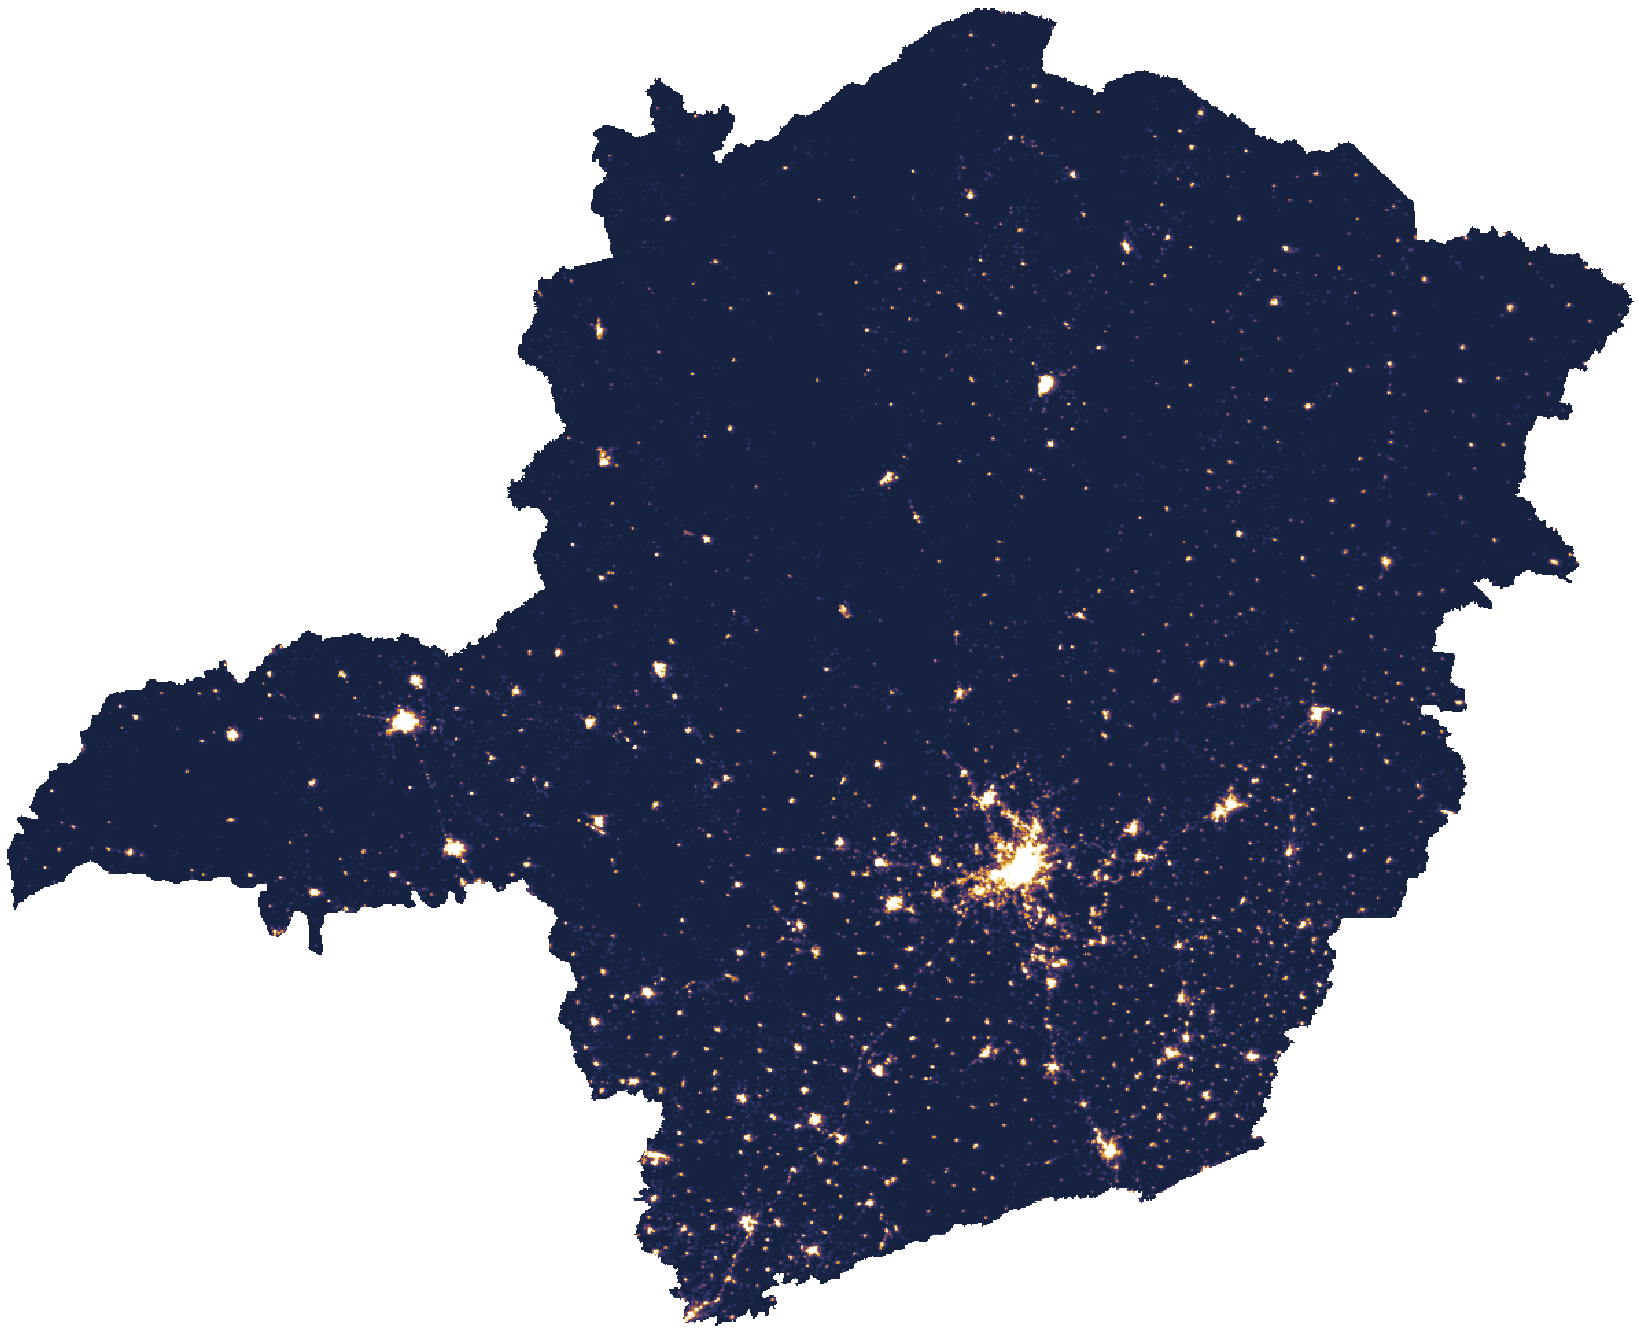
\includegraphics[height=0.96\paperheight]{hero_ntl.png}};
  \begin{scope}[x={($(map.south east)-(map.south west)$)},y={($(map.north west)-(map.south west)$)},shift={(map.south west)}]
    \draw[haze,line width=0.4pt] (0.625,0.345) -- (0.70,0.20) node[anchor=north west,inner sep=1pt,
      font=\fontsize{6.5}{8}\selectfont,text=haze] {Belo Horizonte};
    \draw[haze,line width=0.4pt] (0.245,0.465) -- (0.20,0.33) node[anchor=north,inner sep=1pt,
      font=\fontsize{6.5}{8}\selectfont,text=haze] {Uberlândia};
  \end{scope}
  \node[anchor=south east,font=\fontsize{6}{7}\selectfont,text=haze,align=right] at ($(current page.south east)+(-0.4,0.3)$)
    {VIIRS night lights 2022, one pixel per 1\,km cell};
\end{tikzpicture}
\begin{minipage}{0.47\textwidth}\raggedright
  \eyebrow[glow]{GIS term project \ $\cdot$ \ final presentation}\\[5pt]
  {\fontsize{10.5}{13}\selectfont\bfseries\color{glow}Geospatial Reasoning using LLMs and Generative AI\par}
  \vspace{8pt}
  {\blackfont\fontsize{21}{24}\selectfont\color{white}Reading the economy from space\par}
  \vspace{4pt}
  {\lightfont\fontsize{11}{14}\selectfont\color{white}Municipal GDP from satellite embeddings, text and night lights: what we learned since the mid-term\par}
  \vspace{8pt}
  {\color{glow}\rule{1.6cm}{2.2pt}}\\[7pt]
  {\fontsize{10}{12}\selectfont\bfseries\color{white}Group 2}\\[4pt]
  {\fontsize{8.5}{12}\selectfont\color{white}Hemant \ {\color{haze}(22CS30029)}\\
   Saras Dipak Wagh \ {\color{haze}(22CS30048)}\\
   Pallav Agarwal \ {\color{haze}(22CS30040)}}\\[9pt]
  \href{https://github.com/chadsaras/GIS_Project}{\tikz[baseline=(b.base)]\node[fill=glow,rounded corners=3pt,inner xsep=6pt,
    inner ysep=4pt,font=\bfseries\fontsize{9}{11}\selectfont,text=night] (b)
    {\raisebox{-0.22em}{
\includegraphics[height=1.15em]{github_mark.png}}\ \ github.com/chadsaras/GIS\_Project};}
\end{minipage}
\end{frame}}

%======================== 2. OBJECTIVE =================================
\setstage{1}
\begin{frame}{The question: can free satellite data estimate local GDP?}
\begin{columns}[T,onlytextwidth]
\column{0.42\textwidth}
\centering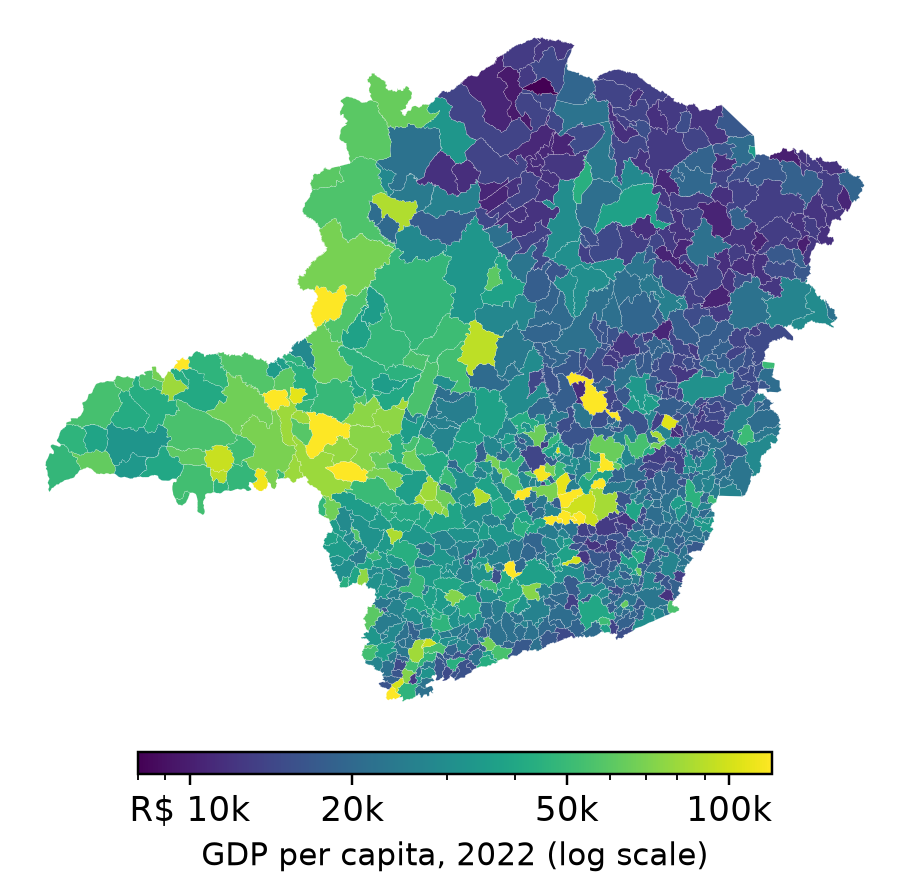
\includegraphics[height=4.9cm]{map_gdp.png}\\[2pt]
{\footnotesize {\blackfont\fontsize{16}{18}\selectfont\color{cgdp}\nGdpRatio$\times$} gap in GDP per capita inside one state}\\
\fnote{\nRichName{} (R\$\,\nRichGdp) vs \nPoorName{} (R\$\,\nPoorGdp)}
\column{0.54\textwidth}
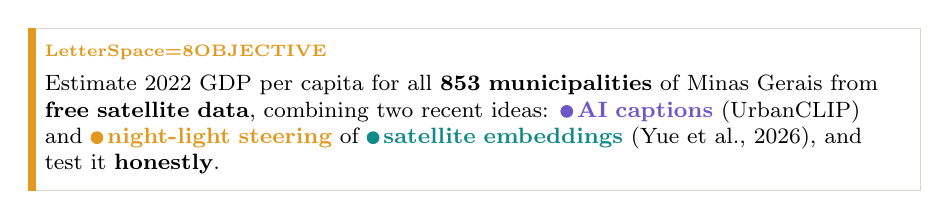
\begin{tikzpicture}
  \node[fill=white,draw=rule,text width=0.9\linewidth,inner sep=6pt,align=left,font=\footnotesize] (g)
    {\eyebrow[cntl]{Objective}\\[3pt]Estimate 2022 GDP per capita for all \textbf{\nMunis{} municipalities} of Minas Gerais from
     \textbf{free satellite data}, combining two recent ideas: \ing{ctxt}{AI captions} (UrbanCLIP) and
     \ing{cntl}{night-light steering} of \ing{cimg}{satellite embeddings} (Yue et al., 2026), and test it \textbf{honestly}.};
  \fill[cntl] (g.north west) rectangle ($(g.south west)+(3pt,0)$);
\end{tikzpicture}\\[8pt]
\eyebrow{Research questions}\\[3pt]
{\renewcommand{\arraystretch}{1.25}\footnotesize
\begin{tabular}{@{}lL{6.1cm}@{}}
\textbf{RQ1} & Does night-light steering improve the estimate?\\
\textbf{RQ2} & Does aligning with text (captions + facts) help?\\
\textbf{RQ3} & Do points of interest and roads add information?\\
\textbf{RQ4} & Does a hybrid with night lights beat the best model?\\
\textbf{RQ5} & Where and why does the model fail?\\
\end{tabular}}
\end{columns}
\end{frame}

%======================== 3. RECAP: PIPELINE ===========================
\setstage{2}\setphase{1}
\begin{frame}{Recap: three learning stages, from pixels to official GDP}
\centering
\begin{tikzpicture}[
  thumbcap/.style={font=\fontsize{7}{8.5}\selectfont,align=center,text=ink,inner sep=1pt},
  flow/.style={-{Stealth[length=2.6mm]},line width=1.4pt,draw=ink}]
  \node[stage=ctxt] (A) at (0,0) {\eyebrow[ctxt]{Stage A}\\[2pt]{\bfseries\small Image--text alignment}\\[1pt]embeddings and captions pulled together};
  \node[stage=cntl] (B) at (4.1,0) {\eyebrow[cntl]{Stage B}\\[2pt]{\bfseries\small Night-light steering}\\[1pt]predict each cell's light, keep the inner layer};
  \node[stage=cgdp] (C) at (8.2,0) {\eyebrow[cgdp]{Stage C}\\[2pt]{\bfseries\small Add up the cells}\\[1pt]per municipality, then predict};
  \node[fill=ink,text=white,text width=2.3cm,minimum height=1.6cm,align=center,inner sep=5pt,font=\footnotesize] (Y) at (11.95,0)
    {{\bfseries\small log GDP\\per capita}\\[2pt]{\color{haze}\nMunis{} municipalities}};
  \draw[flow] (A) -- (B); \draw[flow] (B) -- (C); \draw[flow] (C) -- (Y);
  \node[inner sep=0] (ti) at (-1.0,2.4) {\framed{cimg}{height=1.2cm}{layer_gsed.png}};
  \node[inner sep=0] (tc) at (1.0,2.4) {\framed{ctxt}{height=1.2cm}{caption_tile.png}};
  \node[inner sep=0] (tn) at (4.1,2.4) {\framed{cntl}{height=1.2cm}{layer_ntl.png}};
  \node[inner sep=0] (tg) at (8.2,2.4) {\framed{cgdp}{height=1.2cm}{layer_gdp.png}};
  \node[thumbcap,above=1pt of ti] {\bfseries embeddings};
  \node[thumbcap,above=1pt of tc] {\bfseries captions + facts};
  \node[thumbcap,above=1pt of tn] {\bfseries night lights};
  \node[thumbcap,above=1pt of tg] {\bfseries official GDP};
  \draw[feed=cimg] (ti.south) -- ($(A.north)+(-1.0,0)$);
  \draw[feed=ctxt] (tc.south) -- ($(A.north)+(1.0,0)$);
  \draw[feed=cntl] (tn) -- (B);
  \draw[feed=cgdp] (tg) -- (C);
  \foreach \n/\t/\c in {A/no labels/ctxt,B/cheap proxy label/cntl,C/853 real labels/cgdp}
    \node[below=4pt of \n,font=\bfseries\fontsize{6.5}{8}\selectfont,text=\c] {\MakeUppercase{\t}};
\end{tikzpicture}
\vspace{4pt}

\fnote{Stage A: 64$\to$128 projections, contrastive loss. Stage B: 128$\to$64$\to$\textbf{32}$\to$1, the 32-number layer is the
steered embedding. Stage C: per-cell network, log-sum pooling, 5-seed ensemble. Captions are needed only in training.}
\end{frame}

%======================== 4. RECAP: DATA AND CAPTIONS ==================
\begin{frame}{Recap: six free layers and 10,000 AI captions}
\begin{columns}[c,onlytextwidth]
\column{0.6\textwidth}
\begin{tikzpicture}[
  lname/.style={anchor=west,font=\footnotesize\bfseries,inner sep=0},
  lsrc/.style={anchor=north west,font=\fontsize{6.5}{8}\selectfont,text=muted,inner sep=0,yshift=-2pt}]
  \foreach \img/\c/\name/\src [count=\i from 0] in {
      gsed/cimg/Satellite embeddings/{Google GSED, 64 numbers, 10\,m to 1\,km},
      captions/ctxt/Captioned tiles/{\nCaptions{} Esri tiles, Qwen2.5-VL},
      buildings/ink/Buildings/{Microsoft + OSM footprints},
      roads/cpoi/Roads and POIs/{OpenStreetMap},
      ntl/cntl/Night lights/{VIIRS 2022},
      gdp/cgdp/GDP per capita (target)/{IBGE 2022, official}} {
    \begin{scope}[yshift=\i*0.74cm,cm={1,0.28,-0.62,0.5,(0,0)}]
      \fill[white,draw=\c,line width=0.8pt] (0,0) rectangle (3.0,2.44);
      \node[transform shape,anchor=south west,inner sep=0] at (0,0) {\includegraphics[width=3.0cm,height=2.44cm]{layer_\img.png}};
      \coordinate (r\i) at (3.0,1.22);
    \end{scope}
    \draw[\c,line width=0.5pt] (r\i) -- (r\i -| 4.0,0);
    \fill[\c] (r\i -| 4.0,0) circle (1.5pt);
    \node[lname,text=\c] (n\i) at ($(r\i -| 4.0,0)+(0.15,0.07)$) {\name};
    \node[lsrc] at (n\i.south west) {\src};
  }
\end{tikzpicture}
\column{0.37\textwidth}
\kpi{ink}{\nCells}{kept 1\,km cells, \nMunis{} municipalities}\\[6pt]
\eyebrow[ctxt]{Text, per sampled cell}\\[2pt]
\begin{itemize}\setlength{\itemsep}{2pt}\fontsize{7.5}{9}\selectfont
  \item \textbf{Caption} by Qwen2.5-VL-7B (Kaggle, short prompt after a 200-tile pilot)
  \item \textbf{Fact sentences} from the data: land cover, POIs, roads (no night lights)
  \item \textbf{Cleaning}: filler and claims contradicted by map data removed; RemoteCLIP drops \nClipDropped{} captions
\end{itemize}
\vspace{2pt}
\kpi{okc}{\nKept}{of \nSentences{} caption sentences kept}
\end{columns}
\end{frame}

%======================== 5. RECAP: TEST ===============================
\begin{frame}{Recap: every town is tested in a region never seen}
\begin{columns}[c,onlytextwidth]
\column{0.47\textwidth}
\centering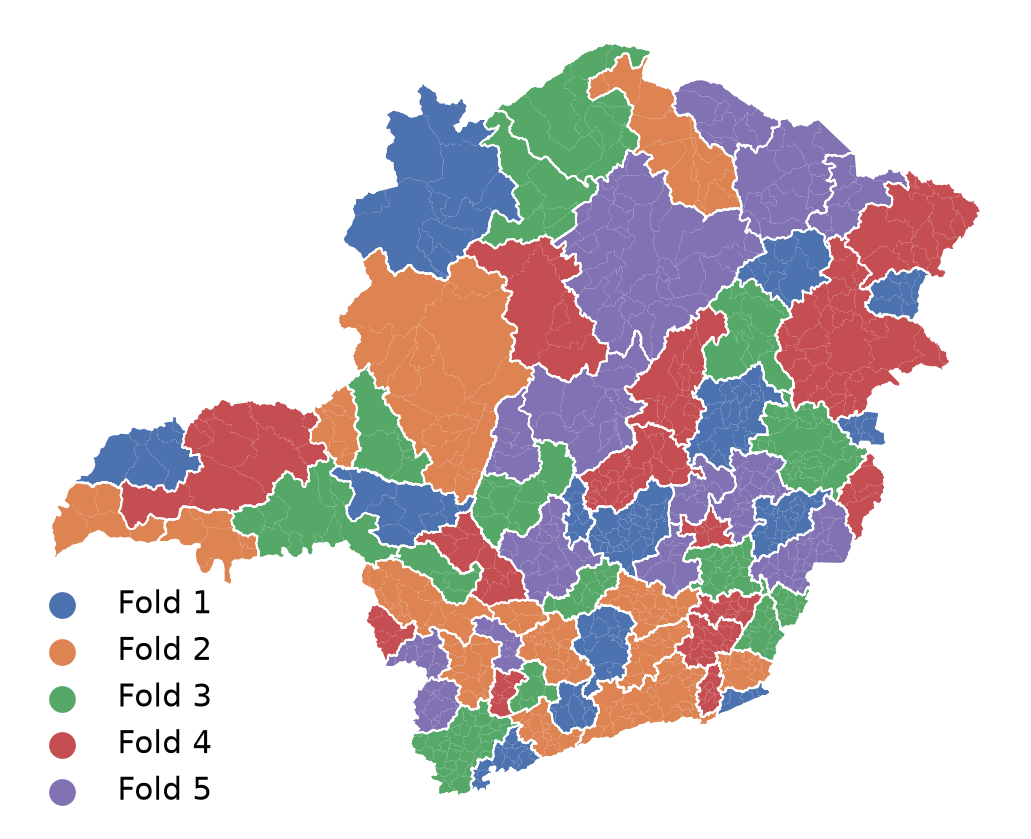
\includegraphics[height=5.3cm]{map_folds.png}\\[-2pt]
\fnote{70 official regions (white outlines) grouped into 5 folds}
\column{0.5\textwidth}
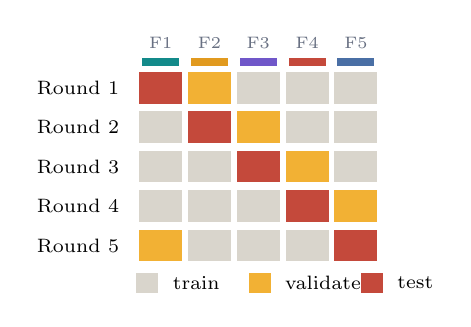
\begin{tikzpicture}[x=0.62cm,y=0.5cm]
  \foreach \c [count=\f from 0] in {cimg,cntl,ctxt,cgdp,cpoi} {
    \fill[\c] (\f+0.12,0.55) rectangle (\f+0.88,0.75);
    \node[font=\fontsize{6.5}{8}\selectfont,text=muted] at (\f+0.5,1.15) {F\the\numexpr\f+1\relax};
  }
  \foreach \r in {0,...,4} {
    \node[anchor=east,font=\fontsize{7}{8}\selectfont] at (-0.15,-\r) {Round \the\numexpr\r+1\relax};
    \pgfmathtruncatemacro\v{mod(\r+1,5)}
    \foreach \f in {0,...,4} {
      \ifnum\f=\r \def\fc{cgdp}\else\ifnum\f=\v \def\fc{glow}\else\def\fc{rule}\fi\fi
      \fill[\fc] (\f+0.06,-\r-0.4) rectangle (\f+0.94,-\r+0.4);
    }
  }
  \foreach \c/\t [count=\k from 0] in {rule/train,glow/validate,cgdp/test} {
    \fill[\c] (\k*2.3,-5.2) rectangle ++(0.45,0.5);
    \node[anchor=west,font=\fontsize{7}{8}\selectfont] at (\k*2.3+0.55,-4.95) {\t};
  }
\end{tikzpicture}\\[8pt]
\begin{itemize}\setlength{\itemsep}{3pt}\footnotesize
  \item Whole regions held out: \textbf{no look-alike neighbour} in training. All three stages retrained each round.
  \item Scalers, tuning and blend weights use training and validation only: \textbf{nothing is tuned on test towns}.
\end{itemize}
\vspace{2pt}
\fnote{Models are compared on the same folds with a block bootstrap over the 70 regions (95\% intervals).}
\end{columns}
\end{frame}

%======================== 6. RECAP: MID-TERM RESULTS ===================
\begin{frame}{Recap: at the mid-term, satellites explained half of GDP}
\begin{columns}[c,onlytextwidth]
\column{0.6\textwidth}
\resizebox{!}{5.0cm}{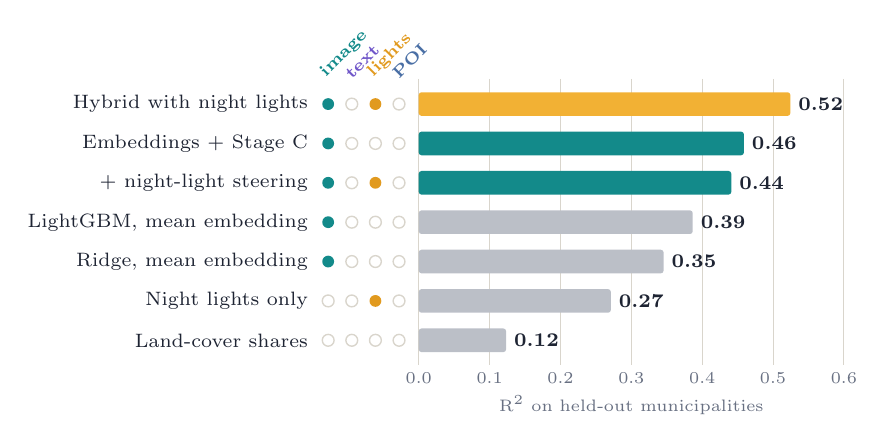
\begin{tikzpicture}[x=1cm,y=1cm,
  lab/.style={font=\fontsize{7.5}{9}\selectfont,text=ink,inner sep=0pt},
  num/.style={font=\bfseries\fontsize{7.5}{9}\selectfont,inner sep=1pt},
  tick/.style={font=\fontsize{6.5}{7.8}\selectfont,text=muted,inner sep=0pt}]
\node[tick,text=cimg,font=\bfseries\fontsize{6}{7}\selectfont,rotate=45,anchor=south west] at (-1.15,0.3) {image};
\node[tick,text=ctxt,font=\bfseries\fontsize{6}{7}\selectfont,rotate=45,anchor=south west] at (-0.85,0.3) {text};
\node[tick,text=cntl,font=\bfseries\fontsize{6}{7}\selectfont,rotate=45,anchor=south west] at (-0.55,0.3) {lights};
\node[tick,text=cpoi,font=\bfseries\fontsize{6}{7}\selectfont,rotate=45,anchor=south west] at (-0.25,0.3) {POI};
\draw[rule,line width=0.4pt] (0.00,0.32) -- (0.00,-3.32);
\node[tick,anchor=north] at (0.00,-3.40) {0.0};
\draw[rule,line width=0.4pt] (0.90,0.32) -- (0.90,-3.32);
\node[tick,anchor=north] at (0.90,-3.40) {0.1};
\draw[rule,line width=0.4pt] (1.80,0.32) -- (1.80,-3.32);
\node[tick,anchor=north] at (1.80,-3.40) {0.2};
\draw[rule,line width=0.4pt] (2.70,0.32) -- (2.70,-3.32);
\node[tick,anchor=north] at (2.70,-3.40) {0.3};
\draw[rule,line width=0.4pt] (3.60,0.32) -- (3.60,-3.32);
\node[tick,anchor=north] at (3.60,-3.40) {0.4};
\draw[rule,line width=0.4pt] (4.50,0.32) -- (4.50,-3.32);
\node[tick,anchor=north] at (4.50,-3.40) {0.5};
\draw[rule,line width=0.4pt] (5.40,0.32) -- (5.40,-3.32);
\node[tick,anchor=north] at (5.40,-3.40) {0.6};
\node[tick,anchor=north] at (2.70,-3.70) {R\textsuperscript{2} on held-out municipalities};
\node[lab,anchor=east] at (-1.4,-0.00) {Hybrid with night lights};
\path[fill=cimg] (-1.15,-0.00) circle (0.075);
\path[draw=rule,line width=0.5pt,fill=white] (-0.85,-0.00) circle (0.075);
\path[fill=cntl] (-0.55,-0.00) circle (0.075);
\path[draw=rule,line width=0.5pt,fill=white] (-0.25,-0.00) circle (0.075);
\fill[glow,rounded corners=1pt] (0,-0.15) rectangle (4.72,0.15);
\node[num,anchor=west,text=ink] at (4.78,-0.00) {0.52};
\node[lab,anchor=east] at (-1.4,-0.50) {Embeddings + Stage C};
\path[fill=cimg] (-1.15,-0.50) circle (0.075);
\path[draw=rule,line width=0.5pt,fill=white] (-0.85,-0.50) circle (0.075);
\path[draw=rule,line width=0.5pt,fill=white] (-0.55,-0.50) circle (0.075);
\path[draw=rule,line width=0.5pt,fill=white] (-0.25,-0.50) circle (0.075);
\fill[cimg,rounded corners=1pt] (0,-0.65) rectangle (4.13,-0.35);
\node[num,anchor=west,text=ink] at (4.19,-0.50) {0.46};
\node[lab,anchor=east] at (-1.4,-1.00) {+ night-light steering};
\path[fill=cimg] (-1.15,-1.00) circle (0.075);
\path[draw=rule,line width=0.5pt,fill=white] (-0.85,-1.00) circle (0.075);
\path[fill=cntl] (-0.55,-1.00) circle (0.075);
\path[draw=rule,line width=0.5pt,fill=white] (-0.25,-1.00) circle (0.075);
\fill[cimg,rounded corners=1pt] (0,-1.15) rectangle (3.97,-0.85);
\node[num,anchor=west,text=ink] at (4.03,-1.00) {0.44};
\node[lab,anchor=east] at (-1.4,-1.50) {LightGBM, mean embedding};
\path[fill=cimg] (-1.15,-1.50) circle (0.075);
\path[draw=rule,line width=0.5pt,fill=white] (-0.85,-1.50) circle (0.075);
\path[draw=rule,line width=0.5pt,fill=white] (-0.55,-1.50) circle (0.075);
\path[draw=rule,line width=0.5pt,fill=white] (-0.25,-1.50) circle (0.075);
\fill[muted!45,rounded corners=1pt] (0,-1.65) rectangle (3.48,-1.35);
\node[num,anchor=west,text=ink] at (3.54,-1.50) {0.39};
\node[lab,anchor=east] at (-1.4,-2.00) {Ridge, mean embedding};
\path[fill=cimg] (-1.15,-2.00) circle (0.075);
\path[draw=rule,line width=0.5pt,fill=white] (-0.85,-2.00) circle (0.075);
\path[draw=rule,line width=0.5pt,fill=white] (-0.55,-2.00) circle (0.075);
\path[draw=rule,line width=0.5pt,fill=white] (-0.25,-2.00) circle (0.075);
\fill[muted!45,rounded corners=1pt] (0,-2.15) rectangle (3.11,-1.85);
\node[num,anchor=west,text=ink] at (3.17,-2.00) {0.35};
\node[lab,anchor=east] at (-1.4,-2.50) {Night lights only};
\path[draw=rule,line width=0.5pt,fill=white] (-1.15,-2.50) circle (0.075);
\path[draw=rule,line width=0.5pt,fill=white] (-0.85,-2.50) circle (0.075);
\path[fill=cntl] (-0.55,-2.50) circle (0.075);
\path[draw=rule,line width=0.5pt,fill=white] (-0.25,-2.50) circle (0.075);
\fill[muted!45,rounded corners=1pt] (0,-2.65) rectangle (2.44,-2.35);
\node[num,anchor=west,text=ink] at (2.50,-2.50) {0.27};
\node[lab,anchor=east] at (-1.4,-3.00) {Land-cover shares};
\path[draw=rule,line width=0.5pt,fill=white] (-1.15,-3.00) circle (0.075);
\path[draw=rule,line width=0.5pt,fill=white] (-0.85,-3.00) circle (0.075);
\path[draw=rule,line width=0.5pt,fill=white] (-0.55,-3.00) circle (0.075);
\path[draw=rule,line width=0.5pt,fill=white] (-0.25,-3.00) circle (0.075);
\fill[muted!45,rounded corners=1pt] (0,-3.15) rectangle (1.11,-2.85);
\node[num,anchor=west,text=ink] at (1.17,-3.00) {0.12};
\end{tikzpicture}
}\\[2pt]
\fnote{R\textsuperscript{2} on held-out municipalities. Dots: ingredients each model uses. Hybrid = best model blended with night lights.}
\column{0.37\textwidth}
\eyebrow{RQ status at the mid-term}\\[4pt]
\chip{muted}{RQ1 STEERING} \ {\footnotesize no clear effect}\\[3pt]
\chip{ctxt}{RQ2 TEXT} \ {\footnotesize largest gain, borderline}\\[3pt]
\chip{muted}{RQ3 POI, ROADS} \ {\footnotesize nothing added}\\[3pt]
\chip{cntl}{RQ4 HYBRID} \ {\footnotesize best, not significant}\\[3pt]
\chip{rule}{\color{muted}RQ5 FAILURES} \ {\footnotesize not answered}\\[8pt]
\eyebrow[cgdp]{Open at the mid-term}\\[2pt]
{\footnotesize Is the result \textbf{reproducible}? How good are the \textbf{captions}? \textbf{Where and why} does it fail?
What did each part \textbf{learn}? Does it work \textbf{elsewhere}?}\\[4pt]
\fnote{Lesson already then: a calibration fix (\nCalibGain{} error) mattered more than steering (backup B2).}
\end{columns}
\end{frame}

%======================== 7. SINCE THE MID-TERM ========================
\setphase{0}
\begin{frame}{Since the mid-term: seven questions, seven pieces of work}
\centering
{\renewcommand{\arraystretch}{1.42}\fontsize{7.8}{9.4}\selectfont
\begin{tabular}{@{}cL{3.8cm}L{4.8cm}L{4.5cm}@{}}
\eyebrow{\#} & \eyebrow{Question} & \eyebrow{Work done} & \eyebrow[okc]{Answer}\\[-3pt]
\midrule
1 & Is the result reproducible? & Full rerun from a fresh clone and data folder & Same verdicts; text gain shrinks\\
2 & How good are the AI captions? & Blind audit of 300 captions, 1{,}801 sentences & \nAuditRaw{} have a false claim, \nAuditClean{} after cleaning\\
3 & Where does it fail? (RQ5) & Maps, ten largest misses, reasons & Mines, steel mills, commuter towns\\
4 & Why does it fail? (RQ5) & Error regression, LOWESS, Moran's I, seeds & Errors rise with income, half as fast as night lights\\
5 & Did each stage do its job? & Stage A/B diagnostics, neighbour check & Yes, but steering does not reach GDP\\
6 & What did the text learn? & Nearest captions, rich-vs-poor word contrast & Text reads the state's economic geography\\
7 & Does it work elsewhere? & São Paulo, models applied unchanged & Satellites R\textsuperscript{2} \nSpR, night lights \nSpNtlR\\
\end{tabular}}\par\vspace{8pt}
\fnote{Also since the mid-term: a 12-page report, results frozen (tag v1.0-results), a one-command rerun script and a data release.}
\end{frame}

%======================== 8. CAPTION AUDIT =============================
\setstage{3}\setphase{2}
\begin{frame}{Blind audit: a third of AI captions hold a false claim}
\begin{columns}[T,onlytextwidth]
\column{0.3\textwidth}
\eyebrow{Method}\\[3pt]
\begin{enumerate}\setlength{\itemsep}{2pt}\fontsize{7.5}{9}\selectfont
  \item 300 random captions, \textbf{1{,}801 sentences}
  \item Each sentence labelled \textbf{correct}, \textbf{false} or \textbf{vague}, with the tile in view
  \item Labeller \textbf{blind} to what cleaning removed
  \item Raw and cleaned scores from the same labels; Wilson 95\% intervals
\end{enumerate}
\vspace{3pt}
\fnote{Labels: 1{,}440 correct, 235 vague, 126 false. Labelled by an LLM (Claude); a human check is still open.}
\column{0.36\textwidth}
\eyebrow{Captions with $\geq$1 false claim}\\[6pt]
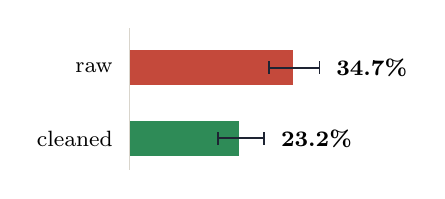
\begin{tikzpicture}[x=0.06cm,y=1cm]
  \foreach \v/\lo/\hi/\lab/\c [count=\i] in {34.7/29.5/40.2/raw/cgdp,23.2/18.7/28.5/cleaned/okc} {
    \node[anchor=east,font=\footnotesize] at (-1.5,-\i*0.9) {\lab};
    \fill[\c] (0,-\i*0.9-0.22) rectangle (\v,-\i*0.9+0.22);
    \draw[ink,line width=0.7pt] (\lo,-\i*0.9) -- (\hi,-\i*0.9);
    \draw[ink,line width=0.7pt] (\lo,-\i*0.9-0.08) -- ++(0,0.16); \draw[ink,line width=0.7pt] (\hi,-\i*0.9-0.08) -- ++(0,0.16);
    \node[anchor=west,font=\bfseries\footnotesize] at (\hi+1.5,-\i*0.9) {\v\%};
  }
  \draw[rule] (0,-0.4) -- (0,-2.2);
\end{tikzpicture}\\[6pt]
{\footnotesize Only 7\% of sentences are false, but a caption has about six, so a third of captions contain one.}
\column{0.3\textwidth}
\eyebrow{How well cleaning works}\\[4pt]
\kpi{okc}{\nAuditRecall}{of false sentences removed (recall)}\\[5pt]
\kpi{cntl}{\nAuditPrecision}{of removed sentences were false or vague (precision)}\\[6pt]
\eyebrow[cgdp]{Typical false claims}\\[1pt]
{\fontsize{7.2}{8.6}\selectfont ``no buildings'' next to farmhouses; ``farmland'' on scrub; ``mining'' on centre-pivot fields; ponds that are not there}
\end{columns}
\end{frame}

%======================== 10. RQ5: MAPS ================================
\setstage{4}
\begin{frame}{RQ5: predictions follow the map, but are pulled to the middle}
\begin{columns}[T,onlytextwidth]
\column{0.28\textwidth}\centering
\eyebrow[cgdp]{Official}\\[2pt]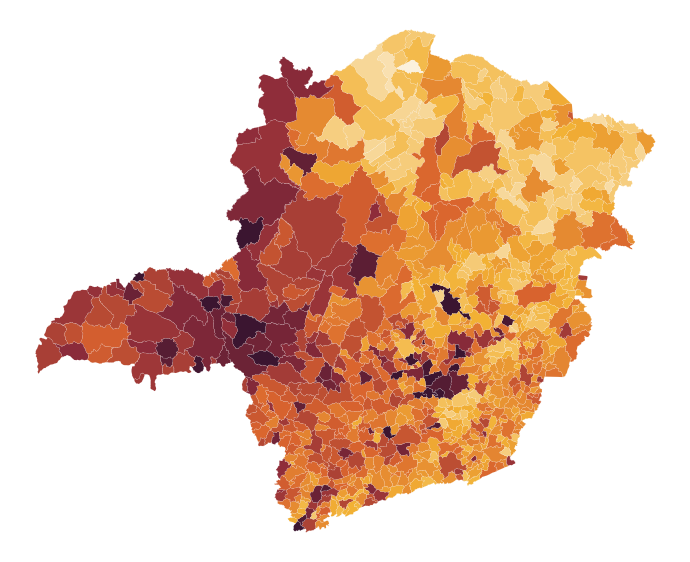
\includegraphics[width=\linewidth]{map_official.png}
\column{0.28\textwidth}\centering
\eyebrow[cgdp]{Predicted (hybrid)}\\[2pt]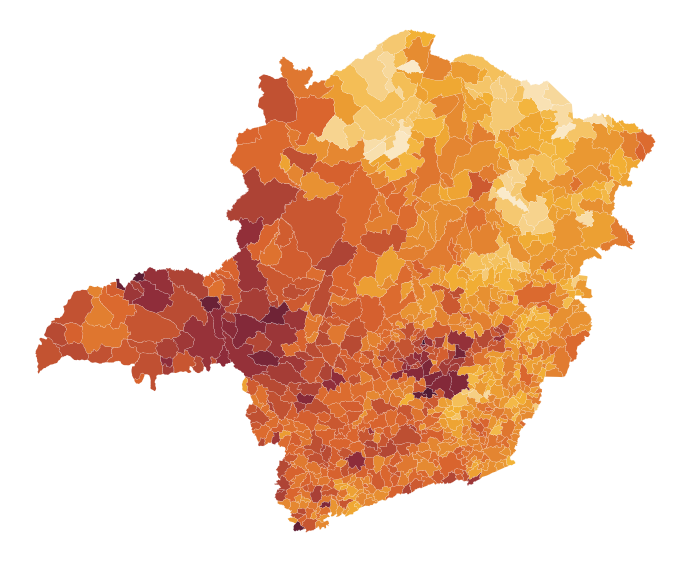
\includegraphics[width=\linewidth]{map_predicted.png}
\column{0.28\textwidth}\centering
\eyebrow{Error}\\[2pt]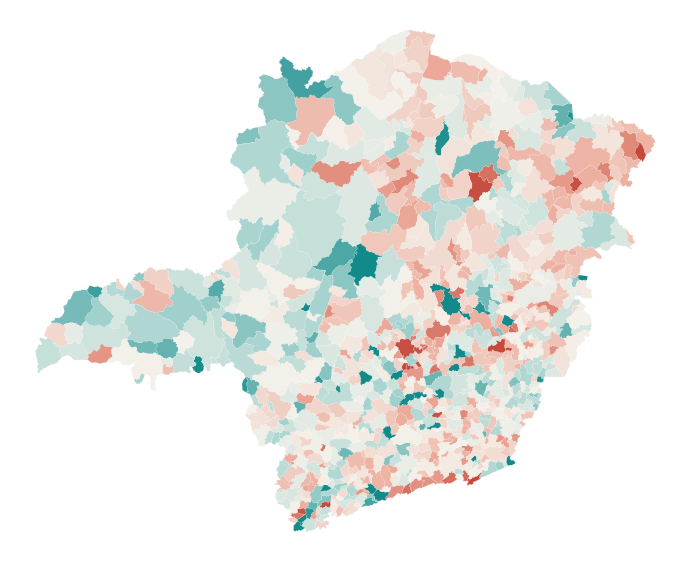
\includegraphics[width=\linewidth]{map_error.png}
\column{0.12\textwidth}
\end{columns}
\begin{columns}[T,onlytextwidth]
\column{0.56\textwidth}\centering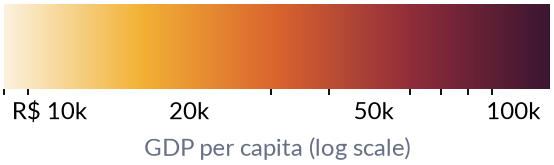
\includegraphics[width=0.5\linewidth]{cbar_gdp.png}
\column{0.28\textwidth}\centering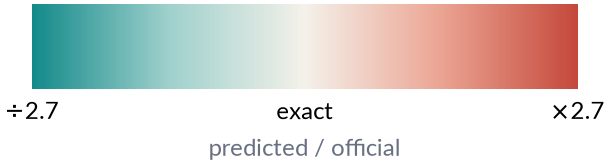
\includegraphics[width=0.85\linewidth]{cbar_err.png}
\column{0.12\textwidth}
\end{columns}
\vspace{8pt}
\begin{columns}[T,onlytextwidth]
\column{0.24\textwidth}
{\blackfont\fontsize{20}{22}\selectfont\color{ink}\nWithinHalf}\\{\fontsize{7}{8.5}\selectfont\color{muted}of municipalities predicted within a factor 1.5 of official}
\column{0.74\textwidth}
\footnotesize \textcolor{cimg}{\textbf{Under-predicted:}} rich agribusiness and mining towns (west, centre).\\[2pt]
\textcolor{cgdp}{\textbf{Over-predicted:}} small public-sector and commuter towns.\\[2pt]
\fnote{Every value is out-of-sample: each town predicted in the round where its region was held out.}
\end{columns}
\end{frame}

%======================== 11. RQ5: MISSES ==============================
\begin{frame}{RQ5: the biggest misses are mines and steel mills}
\begin{columns}[c,onlytextwidth]
\column{0.5\textwidth}
\centering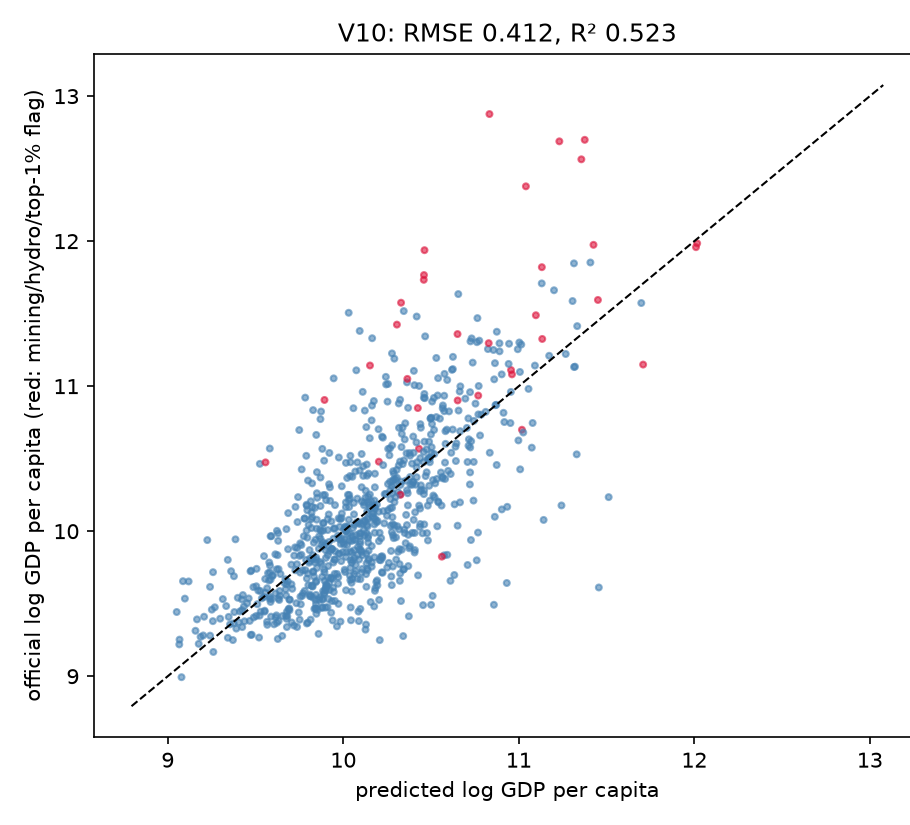
\includegraphics[height=5.0cm]{scatter_v10.png}\\[-1pt]
\fnote{Hybrid, 853 test predictions; red = flagged (industry over 60\% of the economy, or top 1\%).}
\column{0.47\textwidth}
\eyebrow{Ten largest gaps}\\[2pt]
{\renewcommand{\arraystretch}{1.0}\fontsize{7.5}{9}\selectfont
\begin{tabular}{@{}lrl@{}}
\toprule
Municipality & gap & likely reason \\
\midrule
Catas Altas & $-2.04$ & {\color{cimg}\bfseries iron-ore mine} \\
Santa Cruz de Minas & $+1.84$ & {\color{cgdp}\bfseries tiny commuter town} \\
Ressaquinha & $-1.48$ & {\color{cimg}\bfseries large plant} \\
Conceição do Mato Dentro & $-1.48$ & {\color{cimg}\bfseries iron-ore mine} \\
S.\ Gonçalo do Rio Abaixo & $-1.46$ & {\color{cimg}\bfseries iron-ore mine} \\
Mário Campos & $+1.37$ & {\color{cgdp}\bfseries BH commuter town} \\
Itatiaiuçu & $-1.34$ & {\color{cimg}\bfseries iron-ore mine} \\
Extrema & $-1.32$ & {\color{cimg}\bfseries logistics hub} \\
Ouro Branco & $-1.31$ & {\color{cimg}\bfseries steel mill} \\
Chiador & $+1.29$ & {\color{cgdp}\bfseries public-sector town} \\
\bottomrule
\end{tabular}}\\[3pt]
\fnote{Gap = predicted $-$ official (log): $-2.04$ means 7.7$\times$ too low. A few cells make most of the output, while
the tiles show forest and pasture. Reasons are candidates from sector shares.}
\end{columns}
\end{frame}

%======================== 12. RQ5: ERROR STRUCTURE =====================
\begin{frame}{RQ5: errors grow with income, half as fast as night lights}
\begin{columns}[c,onlytextwidth]
\column{0.5\textwidth}
\centering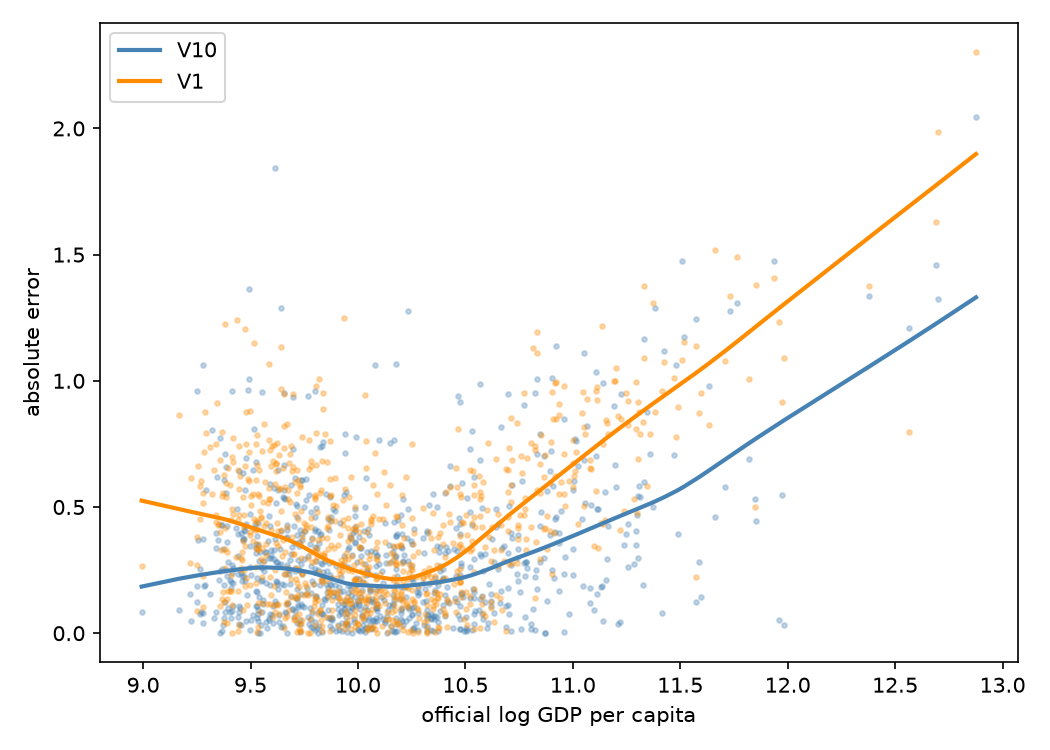
\includegraphics[width=\linewidth]{error_vs_income.png}\\[-2pt]
\fnote{Absolute error against official income, LOWESS. Blue: hybrid; orange: night lights only.}
\column{0.46\textwidth}
\kpi{ink}{\nSlopeV{} \ {\fontsize{12}{14}\selectfont\color{muted}vs} \ \nSlopeNtl}{extra error per log point of income, hybrid vs night lights}\\[8pt]
\kpi{ink}{\nMoranV{} \ {\fontsize{12}{14}\selectfont\color{muted}vs} \ \nMoranNtl}{Moran's I of errors: still clustered in space, half as much}\\[8pt]
\kpi{cgdp}{$\rho = \nUncRho$}{spread across the 5 training seeds does not predict the error}\\[8pt]
\fnote{Error regression with region-clustered SEs (backup B3): errors rise with income and built-up share, fall with
services share; OSM completeness does not matter.}
\end{columns}
\end{frame}

%======================== 13. STAGE DIAGNOSTICS ========================
\setstage{5}
\begin{frame}{Each stage did its job, yet steering does not reach GDP}
\begin{columns}[T,onlytextwidth]
\column{0.42\textwidth}
\eyebrow[ctxt]{Stage A: image--text alignment}\\[3pt]
{\renewcommand{\arraystretch}{1.2}\fontsize{7.5}{9}\selectfont
\begin{tabular}{@{}lcc@{}}
\toprule
Text used & recall@10 & built-up probe R\textsuperscript{2}\\
\midrule
cleaned captions + facts & 0.52 & 0.67\\
raw captions & 0.35 & 0.68\\
facts only & 0.55 & 0.64\\
\textit{chance} & \textit{0.04} & \\
\bottomrule
\end{tabular}}\\[6pt]
\eyebrow[cntl]{Stage B: night-light prediction}\\[2pt]
{\footnotesize validation R\textsuperscript{2} \textbf{0.75--0.78} for every input (best: raw embeddings)}\\[4pt]
\fnote{Mean over 5 rounds, validation towns. Recall within groups of 256 pairs. 81\% of cells are unlit.}
\column{0.54\textwidth}
\eyebrow{The embedding paper's neighbour check (round 0)}\\[3pt]
{\renewcommand{\arraystretch}{1.2}\fontsize{7.5}{9}\selectfont
\begin{tabular}{@{}lcccc@{}}
\toprule
 & \multicolumn{2}{c}{distance to 100 nearest} & \multicolumn{2}{c}{light gap to them}\\
Reference cell & raw & steered & raw & steered\\
\midrule
Rural pasture & 99\,km & 269\,km & 0.00 & 0.03\\
Small town & 82\,km & 292\,km & 0.66 & \textbf{0.46}\\
Industrial area & 19\,km & 39\,km & 0.22 & 0.22\\
Mining / bare ground & 49\,km & 96\,km & 0.90 & \textbf{0.50}\\
BH suburb & 8\,km & 28\,km & 0.20 & 0.20\\
\bottomrule
\end{tabular}}\\[6pt]
{\footnotesize Steered neighbours are \textbf{farther away but as active or more}: steering does what the paper says.
Yet it adds nothing to GDP (RQ1).}
\end{columns}
\end{frame}

%======================== 14. TEXT EXPLANATIONS ========================
\begin{frame}{The text space speaks the state's economic geography}
\begin{columns}[c,onlytextwidth]
\column{0.4\textwidth}
\centering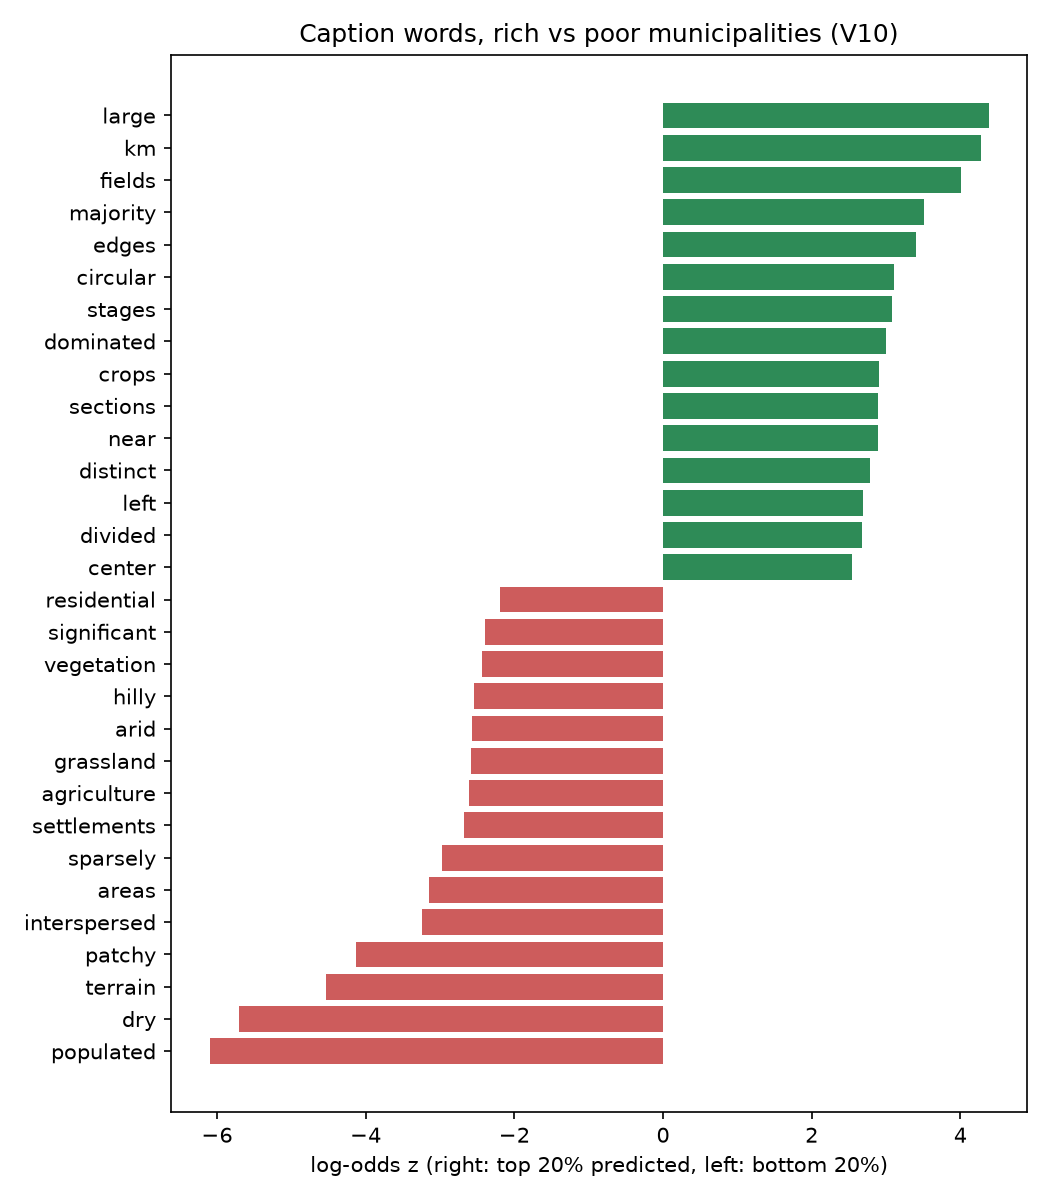
\includegraphics[height=5.6cm]{word_contrast.png}
\column{0.56\textwidth}
\eyebrow[okc]{Richest 20\% predicted}\\[1pt]
{\small \emph{large, fields, circular, crops, divided}: mechanised farming and centre pivots of the Triângulo}\\[8pt]
\eyebrow[cgdp]{Poorest 20\% predicted}\\[1pt]
{\small \emph{sparsely populated, dry, terrain, patchy, arid}: the semi-arid north and Jequitinhonha}\\[8pt]
\eyebrow[ctxt]{Nearest training captions to a town}\\[2pt]
{\footnotesize \textbf{Belo Horizonte} (official 10.82, predicted 10.91): dense grids of red-tiled roofs.\\
\textbf{São João das Missões}, the poorest (8.99 vs 9.08): sparse settlements in dry scrub.\\
\textbf{Conceição do Mato Dentro}, a mine (11.94 vs 10.46): forest and pasture, so the mine stays invisible.}\\[6pt]
\fnote{Word contrast: log-odds with informative Dirichlet prior (Monroe et al., 2008). Values: log GDP per capita.}
\end{columns}
\end{frame}

%======================== 15. TRANSFER: SAO PAULO ======================
\setstage{6}
\begin{frame}{Trained in Minas Gerais, it still works in São Paulo}
\begin{columns}[T,onlytextwidth]
\column{0.32\textwidth}\centering
\eyebrow[cgdp]{Official, IBGE 2022}\\[2pt]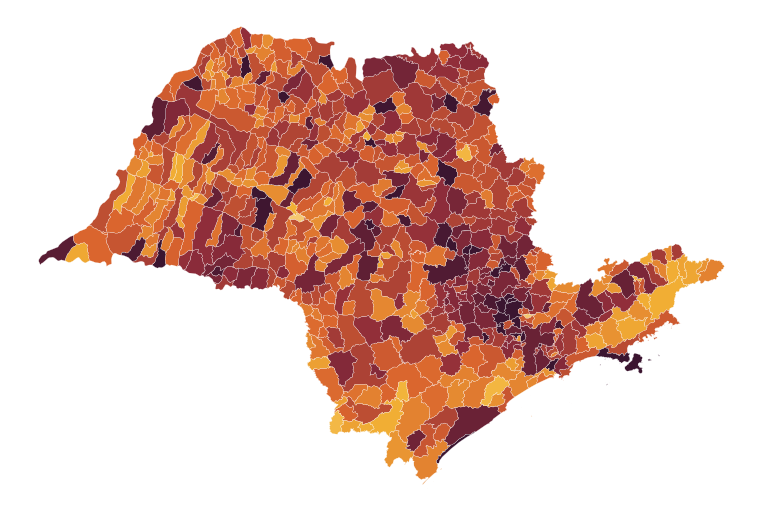
\includegraphics[width=\linewidth]{sp_official.png}
\column{0.32\textwidth}\centering
\eyebrow[cimg]{Predicted, never trained on SP}\\[2pt]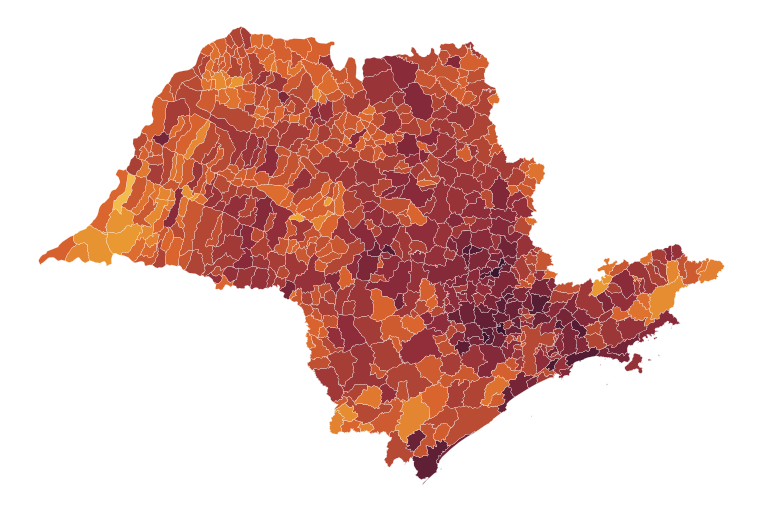
\includegraphics[width=\linewidth]{sp_predicted.png}\\[4pt]
\hspace*{-1.05\linewidth}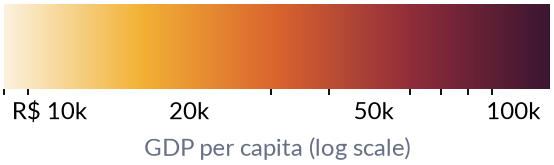
\includegraphics[width=0.95\linewidth]{cbar_gdp.png}
\column{0.32\textwidth}
\eyebrow{R\textsuperscript{2} against official GDP}\\[6pt]
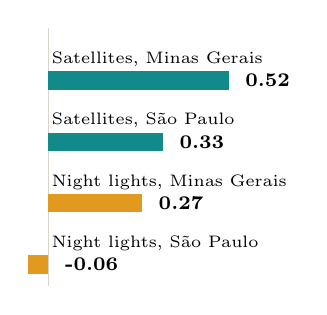
\begin{tikzpicture}[x=4.4cm,y=0.78cm]
  \draw[rule] (0,0.1) -- (0,-4.1);
  \foreach \v/\lab/\c [count=\i] in {0.52/{Satellites, Minas Gerais}/cimg,0.33/{Satellites, São Paulo}/cimg,
                                     0.27/{Night lights, Minas Gerais}/cntl,-0.06/{Night lights, São Paulo}/cntl} {
    \node[anchor=south west,font=\fontsize{6.5}{8}\selectfont,inner sep=1pt] at (0,-\i+0.42) {\lab};
    \fill[\c] (0,-\i+0.4) rectangle (\v,-\i+0.1);
    \node[anchor=west,font=\bfseries\fontsize{7.5}{9}\selectfont] at ({max(\v,0)+0.02},-\i+0.25) {\v};
  }
\end{tikzpicture}\\[4pt]
\fnote{\nSpMunis{} municipalities, all models and scalers from Minas Gerais, nothing refitted. Rank agreement
\textbf{\nSpRho} (night lights \nSpNtlRho); \nSpWithin{} within a factor 1.5. Predicted activity matches SP's
real night lights (R\textsuperscript{2} \nSpAct).}
\end{columns}
\end{frame}

%======================== 16. ANSWERS AND LIMITS ======================
\setstage{7}\setphase{0}
\begin{frame}{Answers to the five questions, and the limits}
\begin{columns}[T,onlytextwidth]
\column{0.53\textwidth}
\eyebrow{Research questions: mid-term $\to$ final}\\[4pt]
{\renewcommand{\arraystretch}{1.32}\small
\begin{tabular}{@{}L{3.0cm}L{3.9cm}@{}}
RQ1 \ night-light steering & \chip{muted}{NO CLEAR EFFECT}\\
RQ2 \ text (captions) & \chip{ctxt}{SMALL GAIN, NOT ROBUST}\\
RQ3 \ POIs and roads & \chip{muted}{NOTHING ADDED}\\
RQ4 \ hybrid & \chip{cntl}{BEST, NOT SIGNIFICANT}\\
RQ5 \ where it fails & \chip{cgdp}{MINES, STEEL, COMMUTER TOWNS}\\
\textit{Beyond}: a new state & \chip{okc}{SATELLITES TRAVEL, LIGHTS DO NOT}\\
\end{tabular}}\\[6pt]
\fnote{Changed since the mid-term: RQ2 (from ``largest gain'' to ``not robust''), RQ5 and the transfer answered.}
\column{0.43\textwidth}
\eyebrow{Limits}\\[3pt]
\begin{itemize}\setlength{\itemsep}{3pt}\footnotesize
  \item GSED is frozen: text can reorganise, not add, image information.
  \item Caption audit labelled by an LLM, one labeller, no agreement score yet.
  \item Stage C was revised after the first test results (choices made on validation).
  \item Trained on one state, tested on one more; other countries and years untested.
  \item Satellites cannot see the value of mines or industry.
\end{itemize}
\end{columns}
\end{frame}

%======================== 19. CLOSING (night) ==========================
{\setbeamertemplate{background}{\nightbg}
\begin{frame}[plain]
\begin{tikzpicture}[remember picture,overlay]
  \node[anchor=east,inner sep=0,opacity=0.55] at ($(current page.east)+(0.3,0)$)
    {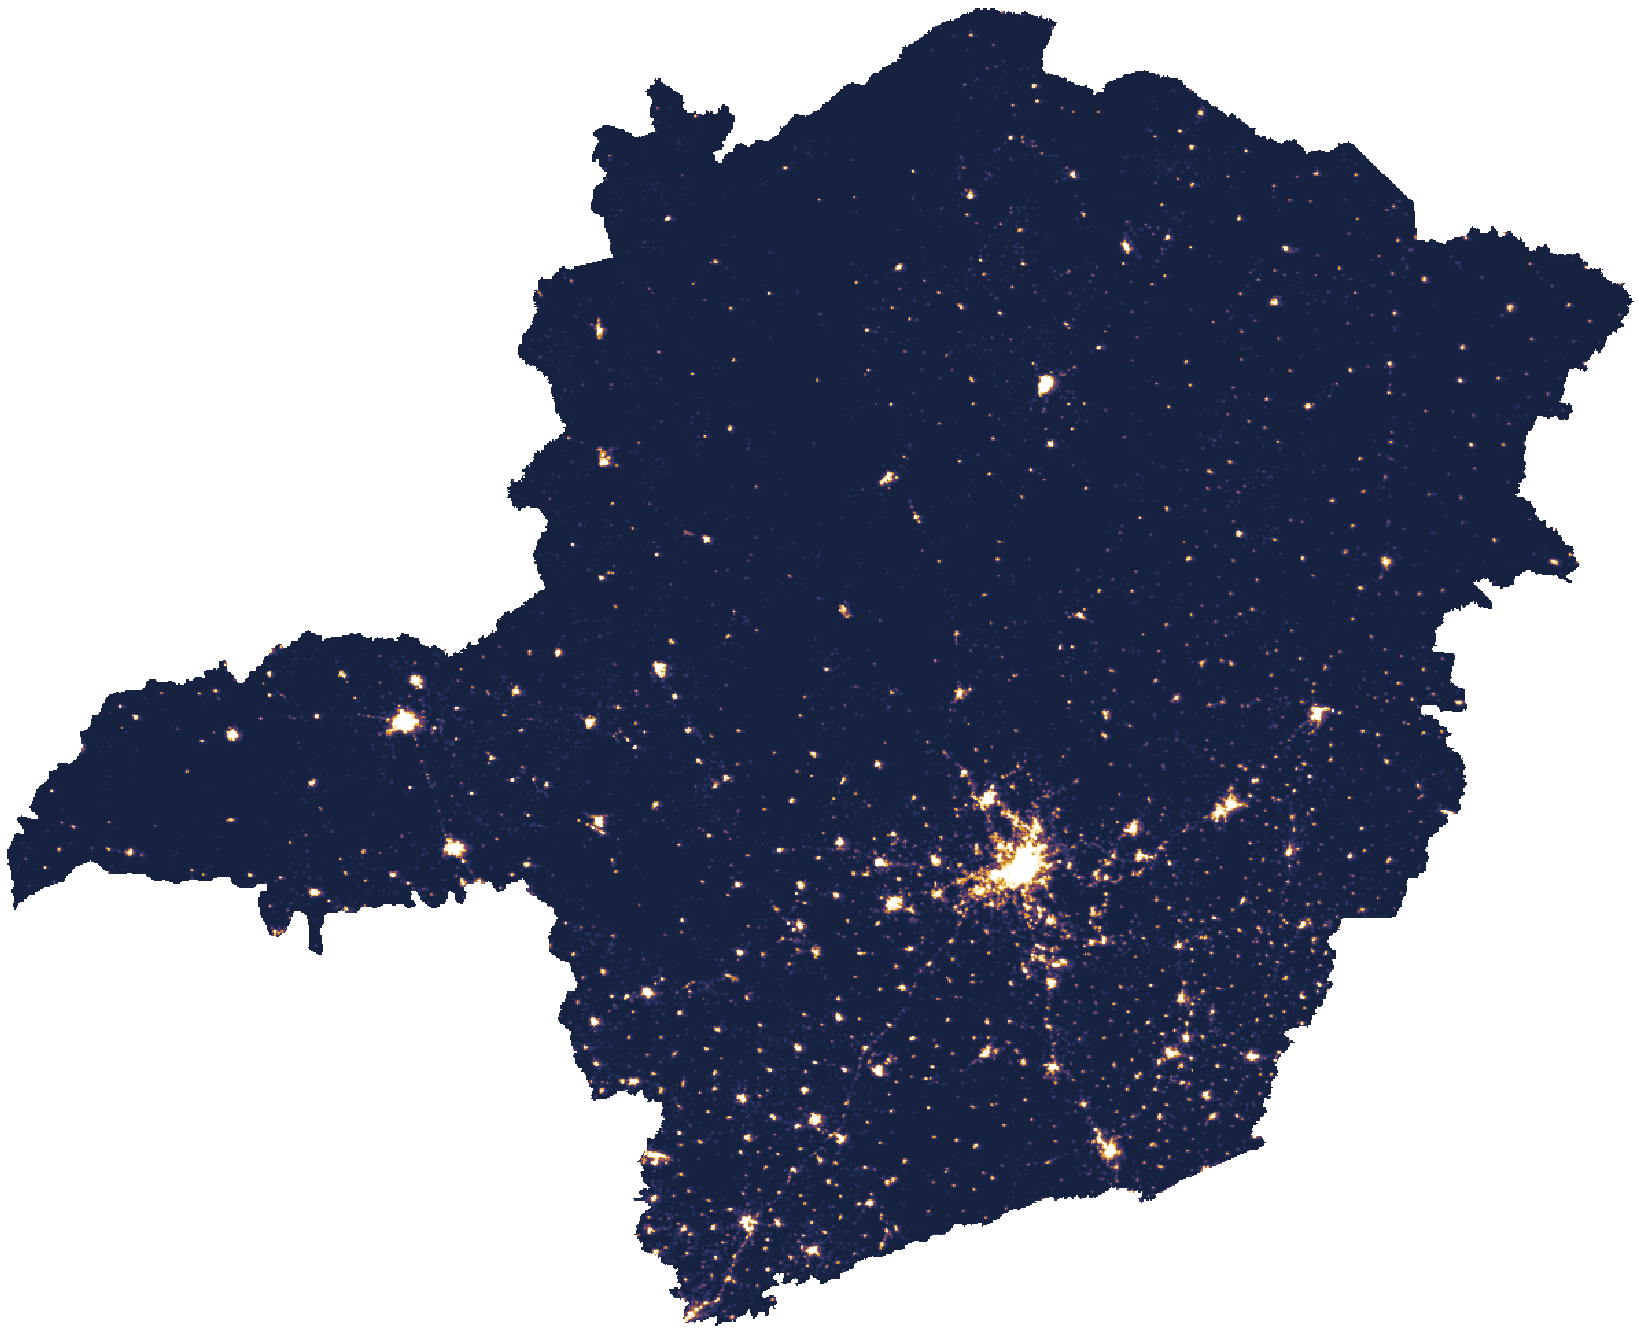
\includegraphics[height=0.9\paperheight]{hero_ntl.png}};
\end{tikzpicture}
\begin{minipage}{0.66\textwidth}\raggedright
\eyebrow[glow]{Take-away}\\[6pt]
{\blackfont\fontsize{15}{19}\selectfont\color{white}Free satellite data explain half of local income differences, the result survives a full rerun, and it travels to a new state where night lights fail.\par}
\vspace{10pt}
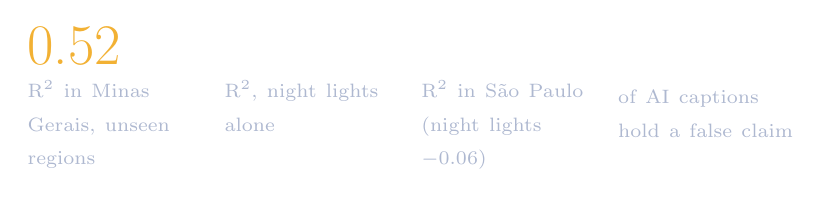
\begin{tikzpicture}[k/.style={anchor=north west,text width=2.3cm,align=left,inner sep=0}]
  \node[k] at (0,0) {{\blackfont\fontsize{22}{24}\selectfont\color{glow}\nHybridR}\\{\fontsize{7}{8.5}\selectfont\color{haze}R\textsuperscript{2} in Minas Gerais, unseen regions}};
  \node[k] at (2.5,0) {{\blackfont\fontsize{22}{24}\selectfont\color{white}\nNtlR}\\{\fontsize{7}{8.5}\selectfont\color{haze}R\textsuperscript{2}, night lights alone}};
  \node[k] at (5.0,0) {{\blackfont\fontsize{22}{24}\selectfont\color{white}\nSpR}\\{\fontsize{7}{8.5}\selectfont\color{haze}R\textsuperscript{2} in São Paulo (night lights \nSpNtlR)}};
  \node[k] at (7.5,0) {{\blackfont\fontsize{22}{24}\selectfont\color{white}\nAuditRaw}\\{\fontsize{7}{8.5}\selectfont\color{haze}of AI captions hold a false claim}};
\end{tikzpicture}
\vspace{10pt}

{\footnotesize\color{haze}Steering, POIs and roads add nothing clear; text adds little.
\textbf{\color{white}Satellites miss what they cannot see:} mines, steel mills and commuter towns.}\\[12pt]
{\blackfont\fontsize{16}{18}\selectfont\color{white}Questions?}\\[3pt]
{\fontsize{7.5}{9}\selectfont\color{haze}github.com/chadsaras/GIS\_Project}
\end{minipage}
\end{frame}}

%======================== B1. TWO IDEAS ================================
\setstage{-1}\setphase{1}
\begin{frame}{Backup: two recent ideas, never tested together}
\centering
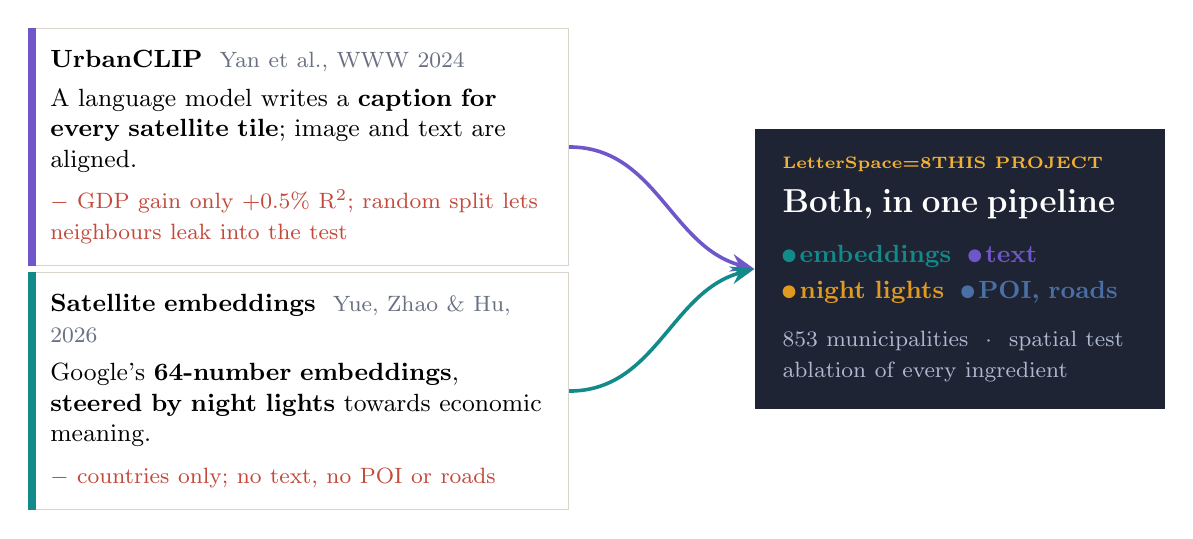
\begin{tikzpicture}[
  card/.style={fill=white,draw=rule,text width=6.3cm,inner sep=8pt,align=left,font=\small},
  arr/.style={-{Stealth[length=3mm]},line width=1.3pt}]
  \node[card] (u) at (0,1.55) {{\bfseries UrbanCLIP} \ \muted{\footnotesize Yan et al., WWW 2024}\\[3pt]
    A language model writes a \textbf{caption for every satellite tile}; image and text are aligned.\\[4pt]
    {\footnotesize\color{cgdp}$-$\ GDP gain only +0.5\% R\textsuperscript{2}; random split lets neighbours leak into the test}};
  \fill[ctxt] (u.north west) rectangle ($(u.south west)+(3pt,0)$);
  \node[card] (e) at (0,-1.55) {{\bfseries Satellite embeddings} \ \muted{\footnotesize Yue, Zhao \& Hu, 2026}\\[3pt]
    Google's \textbf{64-number embeddings}, \textbf{steered by night lights} towards economic meaning.\\[4pt]
    {\footnotesize\color{cgdp}$-$\ countries only; no text, no POI or roads}};
  \fill[cimg] (e.north west) rectangle ($(e.south west)+(3pt,0)$);
  \node[fill=ink,text=white,text width=4.5cm,inner sep=10pt,align=left,font=\small] (o) at (8.4,0)
    {\eyebrow[glow]{This project}\\[5pt]
     {\large\bfseries Both, in one pipeline}\\[7pt]
     \ing{cimg}{embeddings} \ \ing{ctxt}{text}\\[2pt]
     \ing{cntl}{night lights} \ \ing{cpoi}{POI, roads}\\[8pt]
     {\color{haze}\footnotesize \nMunis{} municipalities \ $\cdot$ \ spatial test\\ablation of every ingredient}};
  \draw[arr,ctxt] (u.east) to[out=0,in=165] (o.west);
  \draw[arr,cimg] (e.east) to[out=0,in=195] (o.west);
\end{tikzpicture}
\end{frame}

%======================== B2. CALIBRATION ==============================
\begin{frame}{Backup: calibration mattered more than night-light steering}
\begin{columns}[c,onlytextwidth]
\column{0.46\textwidth}
\centering\resizebox{\linewidth}{!}{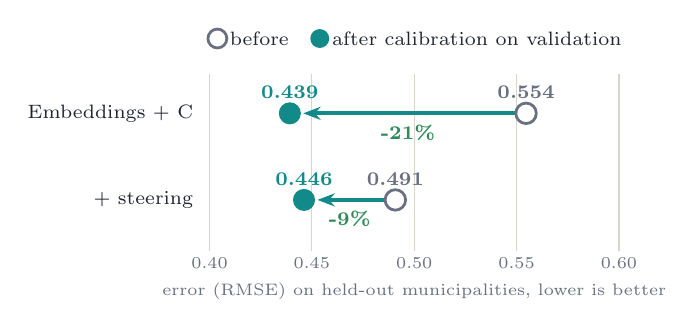
\begin{tikzpicture}[x=1cm,y=1cm,
  lab/.style={font=\fontsize{7.5}{9}\selectfont,text=ink,inner sep=0pt},
  num/.style={font=\bfseries\fontsize{7.5}{9}\selectfont,inner sep=1pt},
  tick/.style={font=\fontsize{6.5}{7.8}\selectfont,text=muted,inner sep=0pt}]
\draw[rule,line width=0.4pt] (0.00,0.5) -- (0.00,-1.75);
\node[tick,anchor=north] at (0.00,-1.83) {0.40};
\draw[rule,line width=0.4pt] (1.30,0.5) -- (1.30,-1.75);
\node[tick,anchor=north] at (1.30,-1.83) {0.45};
\draw[rule,line width=0.4pt] (2.60,0.5) -- (2.60,-1.75);
\node[tick,anchor=north] at (2.60,-1.83) {0.50};
\draw[rule,line width=0.4pt] (3.90,0.5) -- (3.90,-1.75);
\node[tick,anchor=north] at (3.90,-1.83) {0.55};
\draw[rule,line width=0.4pt] (5.20,0.5) -- (5.20,-1.75);
\node[tick,anchor=north] at (5.20,-1.83) {0.60};
\node[tick,anchor=north] at (2.60,-2.15) {error (RMSE) on held-out municipalities, lower is better};
\node[lab,anchor=east] at (-0.2,-0.00) {Embeddings + C};
\draw[-{Stealth[length=2.2mm]},cimg,line width=1.4pt] (3.88,-0.00) -- (1.19,-0.00);
\node[circle,draw=muted,fill=white,line width=1pt,minimum size=2.6mm,inner sep=0pt] at (4.02,-0.00) {};
\node[circle,fill=cimg,minimum size=2.8mm,inner sep=0pt] at (1.02,-0.00) {};
\node[num,text=muted,anchor=south] at (4.02,0.14) {0.554};
\node[num,text=cimg,anchor=south] at (1.02,0.14) {0.439};
\node[num,text=okc,anchor=north] at (2.52,-0.10) {-21\%};
\node[lab,anchor=east] at (-0.2,-1.10) {+ steering};
\draw[-{Stealth[length=2.2mm]},cimg,line width=1.4pt] (2.22,-1.10) -- (1.37,-1.10);
\node[circle,draw=muted,fill=white,line width=1pt,minimum size=2.6mm,inner sep=0pt] at (2.36,-1.10) {};
\node[circle,fill=cimg,minimum size=2.8mm,inner sep=0pt] at (1.20,-1.10) {};
\node[num,text=muted,anchor=south] at (2.36,-0.96) {0.491};
\node[num,text=cimg,anchor=south] at (1.20,-0.96) {0.446};
\node[num,text=okc,anchor=north] at (1.78,-1.20) {-9\%};
\node[circle,draw=muted,fill=white,line width=1pt,minimum size=2.4mm,inner sep=0pt] at (0.1,0.95) {};
\node[lab,anchor=west] at (0.25,0.95) {before};
\node[circle,fill=cimg,minimum size=2.4mm,inner sep=0pt] at (1.4,0.95) {};
\node[lab,anchor=west] at (1.55,0.95) {after calibration on validation};
\end{tikzpicture}
}
\column{0.5\textwidth}
\begin{enumerate}\setlength{\itemsep}{9pt}\small
  \item \textbf{Predictions were over-spread.} A straight-line correction fitted on validation municipalities
        cut error by {\bfseries\color{okc}\nCalibGain}.
  \item \textbf{Honest testing changes conclusions.} Steering looked helpful before the fix; after it, the gain vanished.
  \item \textbf{Disclosed:} the fix was chosen on validation data, but after the first test results were seen.
\end{enumerate}
\end{columns}
\end{frame}

%======================== B3. ERROR REGRESSION =========================
\setphase{2}
\begin{frame}{Backup: what predicts a large error?}
\centering
{\renewcommand{\arraystretch}{1.25}\footnotesize
\begin{tabular}{@{}lcccc@{}}
\toprule
 & \multicolumn{2}{c}{Hybrid (V10)} & \multicolumn{2}{c}{Night lights (V1)}\\
Municipality trait & coef. (SE) & $p$ & coef. (SE) & $p$\\
\midrule
official log GDP per capita & 0.081 (0.035) & 0.02 & 0.190 (0.037) & $<$0.001\\
built-up share & 0.836 (0.473) & 0.08 & 0.791 (0.250) & 0.002\\
services share of the economy & $-$0.285 (0.132) & 0.03 & $-$0.332 (0.123) & 0.007\\
industry share of the economy & 0.185 (0.121) & 0.13 & $-$0.107 (0.102) & 0.29\\
flagged (mining, hydro, top 1\%) & 0.165 (0.090) & 0.07 & 0.272 (0.079) & $<$0.001\\
OSM completeness & $-$0.018 (0.082) & 0.82 & $-$0.099 (0.054) & 0.07\\
\bottomrule
\end{tabular}}\par\vspace{8pt}
\fnote{OLS of absolute error, 853 municipalities, standard errors clustered by immediate region. Sector shares from 2021.
IBGE publishes no data-quality score per municipality, so income and economic structure are used instead.}
\end{frame}

\end{document}
